% Section 2 - Message topics
% Roberto Masocco <roberto.masocco@uniroma2.it>
% May 2, 2026

% ### Message topics ###
\section{Message topics}
\graphicspath{{figs/section2/}}

% --- ROS 2 messages ---
\begin{frame}{ROS 2 messages}
	\justifying
	A message is a \textbg{single data packet} sent over a \textbg{topic}, from \textbg{publisher nodes} to \textbg{subscriber nodes}, with a specific \textbg{QoS policy}.
	\begin{figure}
		\centering
		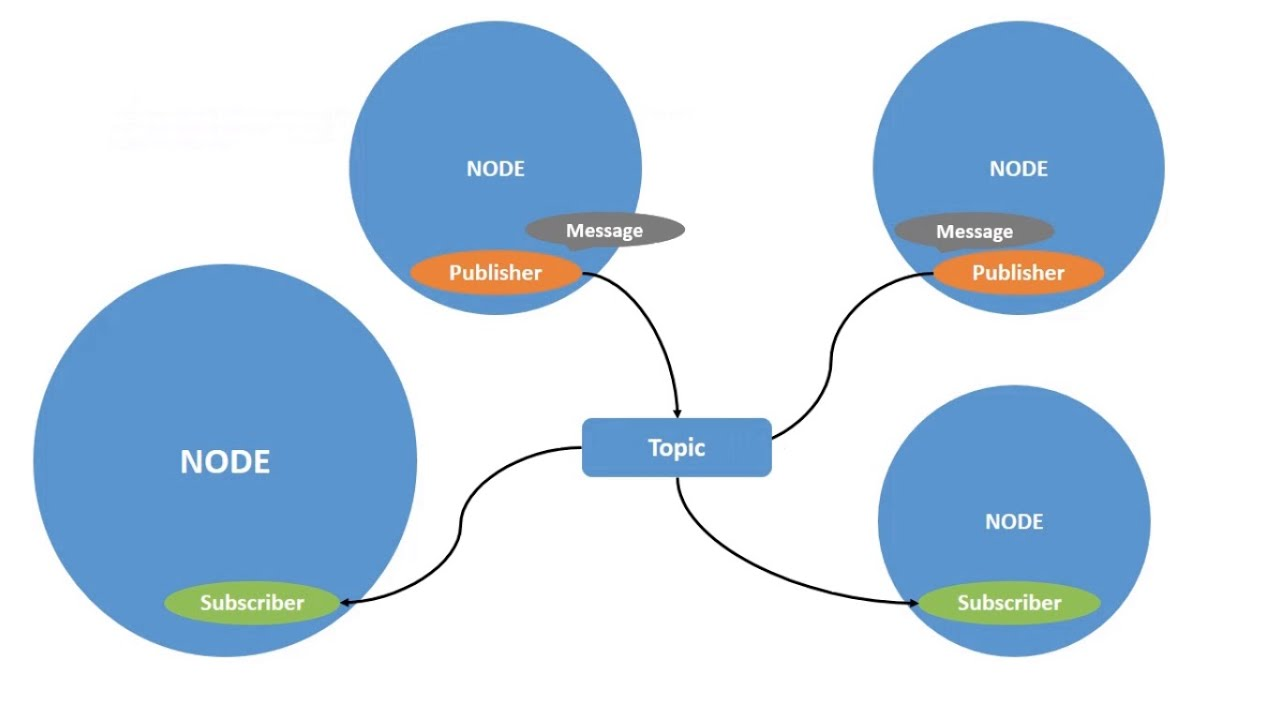
\includegraphics[scale=.16]{ros2Msg.jpg}
		\caption{Example of a topic with multiple publisher and subscriber nodes.}
		\label{fig:msg}
	\end{figure}
  Figure \ref{fig:msg} is also an example of a simple \textbg{node graph}, a pivotal concept in a distributed context.
\end{frame}

% --- Interface files - Messages ---
\begin{frame}[fragile]{Interface files}{Messages}
	\justifying
	Interface files format is \textbg{derived from the DDS standard}, with data types resolved to machine types according to the platform being used\footnote{\href{https://docs.ros.org/en/jazzy/Concepts/About-ROS-Interfaces.html}{\color{blue}\underline{About ROS 2 interfaces}} (ROS 2 Jazzy docs)}.\\
  \medskip
	Message file names end with \texttt{.msg}.\\
  \medskip
	Things start very simply...

	\begin{columns}
		\column{.9\textwidth}
		% Listing: std_msgs/msg/Int64 message definition
		\begin{lstlisting}[language=ros2msg, caption=Definition of the \texttt{std\_msgs/msg/Int64} message.]
int64 data
    \end{lstlisting}

		% Listing: std_msgs/msg/String message definition
		\begin{lstlisting}[language=ros2msg, caption=Definition of the \texttt{std\_msgs/msg/String} message.]
string data
    \end{lstlisting}
	\end{columns}
\end{frame}
\begin{frame}[fragile]{Interface files}{Messages}
	\justifying
	... then escalate quickly!

	\begin{columns}
		\column{.9\textwidth}
		% Listing: sensor_msgs/msg/Image
		\begin{lstlisting}[language=ros2msg, caption=Definition of the \texttt{sensor\_msgs/msg/Image} nested message.]
std_msgs/Header header
# ^ This includes another message type as a sub-structure

uint32 height
uint32 width

string encoding

uint8 is_bigendian
uint32 step
uint8[] data # This specifies a variable-length uint8 array
    \end{lstlisting}
	\end{columns}
\end{frame}
\begin{frame}[fragile]{Interface files}{Messages}
	\justifying
	Special values (\emph{i.e.}, \textbg{constants}) or \textbg{default values} may be specified.

	\begin{columns}
		\column{.9\textwidth}
		% Listing: message with constant
		\begin{lstlisting}[language=ros2msg, caption=Definition of an example message with a constant and a default value.]
int64 MYNUM=1 # Must be of compatible type

int64 number
int64 number_with_default 2
    \end{lstlisting}
	\end{columns}

	They are not bound to any field and will appear as \textbg{special selectable values} in the generated C++/Python (libraries) code.\\
	ROS 2 adds its own \textbg{guidelines}\footnote{\href{https://github.com/IntelligentSystemsLabUTV/ros2-examples/blob/jazzy/interfaces.md}{\color{blue}\underline{ros2-examples/interfaces.md}}}, and installed interfaces can be \textbg{inspected} with\\
  \medskip
	\texttt{ros2 interface show}
\end{frame}

% --- Message topics - Quality of Service ---
\begin{frame}{Message topics}{Quality of Service}
	\justifying
	A \href{https://docs.ros.org/en/jazzy/Concepts/About-Quality-of-Service-Settings.html}{\color{blue}\textbf{\underline{QoS policy}}} for a \textbg{topic} is a data structure with the following attributes.
	\begin{itemize}
		\item \textbg{History} (\emph{keep last N} or \emph{all})
		\item \textbg{Depth} (queue size \emph{N})
		\item \textbg{Reliability} (\emph{best-effort} or \emph{reliable}, default: reliable)
		\item \textbg{Durability} (publishers resend all messages to "late-joiners")
		\item Deadline
		\item Lifespan
		\item Liveliness
		\item Lease duration
	\end{itemize}
\end{frame}
\begin{frame}{Message topics}{Quality of Service}
  \justifying
  \begin{alertblock}{On the structure of a ROS 2 QoS policy}
    \justifying
    The full number of attributes of a ROS 2 QoS policy \textbr{comes from the DDS world}.\\
    \medskip
    The \textbr{DDS} standard defines \textbr{22 QoS settings}, many of which have been \textbr{mapped directly in ROS}, many more have been \textbr{abstracted away by RMW}.\\
    \medskip
    Some of the QoS settings of the \textbr{DDS} \textbr{only provide a notification} that a condition is violated without actively enforcing it (\emph{e.g.}, temporal properties such as deadlines), or \textbr{have never been implemented} by vendors because of obsolescence.\\
    \medskip
    \textbr{ROS 2 inevitably inherited some of this complexity, sometimes unnecessarily.}
  \end{alertblock}
  \textbg{Zenoh simplifies this scenario with a lean implementation:}
  \begin{itemize}
    \item a minimal set of \textbg{core settings} are exposed (see previous marked ones);
    \item some have become \textbg{protocol features} guaranteed by the implementation.
  \end{itemize}
\end{frame}
\begin{frame}{Message topics}{Quality of Service}
  \justifying
  \begin{alertblock}{On ROS QoS profiles}
    \justifying
    \textbr{Since ROS 1}, client libraries have always provided \textbr{QoS profiles for standard scenarios}:
    \begin{itemize}
      \item \texttt{default} (\textbr{reliable}, keep last 10, volatile);
      \item \texttt{sensor\_data} for \textbr{continuous streams of samples} (\textbr{best-effort}, keep last 5, volatile: \textbr{if one is lost, the following ones should make it through}...);
      \item services, parameters, and other ROS internal communications.
    \end{itemize}
    \textbr{ROS QoS profiles have been designed in a past time when ROS was not mature and widespread as it is today. In real scenarios, it is the communication technologies that should be selected, refined, and tuned to guarantee reliability.}
  \end{alertblock}
  \textbg{Zenoh is solving this by supporting many more real-world networks and use cases than the DDS.}
\end{frame}
\begin{frame}{Message topics}{Inspection tools}
  \justifying
  The command line tool \texttt{ros2 topic} can be used to \textbg{inspect topics} and related entities.\\
  It has a lot of \textbg{verbs}, the most important ones are:
  \begin{itemize}
    \item \texttt{list} (list all topics)
    \item \texttt{echo} (print messages to the console)
    \item \texttt{pub} (publish messages from the console)
    \item \texttt{hz} (print publishing rate and statistics)
    \item \texttt{info} (print information about a topic)
    \item \texttt{type} (print the message type)
  \end{itemize}
  each with many useful options.\\
  \textbg{Nodes} can be inspected with the \texttt{ros2 node} command, and its many verbs.
\end{frame}
